\subsection{Exceções}

A linguagem de programação \acs{PHP} 5, introduz o conceito de exceções, e isto traz
uma grande vantagem se comparada a manipulação de erros das versões anteriores
da tecnologia, além disto, você poderá também encontrar similaridades nos
conceitos aplicados ao \acs{PHP} caso tenha conhecimento de outras linguagens, tais
como: \textit{Java} e \textit{C++} \cite{phpObjectsPatternsAndPractice}.

Uma exceção indica que ocorreu uma condição não esperada ou um erro, sendo que,
isto geralmente acontece por conta de um erro de processamento, como por
exemplo: uma atribuição ou leitura de valores incorretos ou obrigatórios em
variáveis locais e propriedades durante a execuçao de um método \cite{learningJava}.

Segundo \citeonline{phpObjectsPatternsAndPractice} uma exceção é um objeto
especial instanciado a partir da classe \textit{Exception}, ou a partir de uma
classe especialista, portanto, estes objetos são projetados para criar e
reportar informações de erro.

Sendo assim, se comparado a forma tradicional de manipulação de erros, as
exceções são uma forma elegante de manipulá-los e tratá-los dentro de uma
aplicação, de acordo com o que foi visto no capítulo que
tratava sobre herança, pode-se extender as funcionalidas da classe
\textit{Exception}, personalizando os seus dados e o seu comportamento \cite{phpMasterWriteCuttingEdgeCode}.

Conforme afirma \citeonline{phpMasterWriteCuttingEdgeCode}, um objeto da classe
\textit{Exception}, irá conter informações referente ao erro que ocorreu, dentre
estas informações estão:

\begin{alineas}
    \item o nome do arquivo;
    \item a linha em que ocorreu o problema;
    \item uma mensagem;
    \item e, opcionalmente, um código de erro.
\end{alineas}

O Quadro \ref{tab:excecao} apresenta os métodos da classe \textit{Exception}
presente na linguagem de programação \acs{PHP}.

% Esta tabela está na p.52] da referencia: phpObjectsPatternsAndPractice
\begin{table}[h!tb]
	\centering
	\setlength{\belowcaptionskip}{9pt}
	\caption{Métodos públicos da classe \textit{Exception}}
	\begin{tabular}{| l | p{0.7\textwidth} |}

		\hline
		\textbf{Método}
		& \textbf{Descrição} \\
		\hline

        \textit{getMessage()}
        & Recupeara uma \textit{string} que foi enviada
        para o construtor.

        \\ \cline{1-2}
        \textit{getCode()}
        & Recupera o código de erro.
        \\ \cline{1-2}

        \textit{getFile()}
        & Recupera o arquivo em que a exceção foi lançada.
        \\ \cline{1-2}

        \textit{getLine()}
        & Recupera o número da linha em que a exceção ocorreu.
        \\ \cline{1-2}

        \textit{getPrevious()}
        & Recupera um objeto de uma exceção.
        \\ \cline{1-2}

        \textit{getTrace()}
        & Recupera um \textit{array} multimensional contendo as chamadas de
        métodos, incluindo: funções membro, classes, arquivos e argumentos. \\
        \cline{1-2}

        \textit{getTraceAsString()}
        & Recupera os dados de \textit{getTrace()} no formato de uma
        \textit{string}.
        \\ \cline{1-2}

        \textit{\_\_toString()}
        & Método mágico executado automaticamente quando um objeto é exibido em
        tela como uma \textit{string}. Sendo assim, retorna uma \textit{string}
        descrevendo os detalhes da exceção.
        \\
        \hline
	\end{tabular}
	\newline
	\newline
	\label{tab:excecao}
	\begin{footnotesize}
		Fonte: adaptado de \cite[p.53]{phpObjectsPatternsAndPractice}
	\end{footnotesize}
\end{table}

\FloatBarrier 	% Este comando impede que as imagens
				% flutuem a partir deste ponto no seu documento


A seguir, será apresentada na Figura \ref{fig:excecao} a manipulação de um erro de
processamento com o uso da classe \textit{Exception}.

\begin{figure}[h!tb]
	\caption{Classe \textit{Exception} da linguagem PHP}
	\label{fig:excecao}

	\centering
	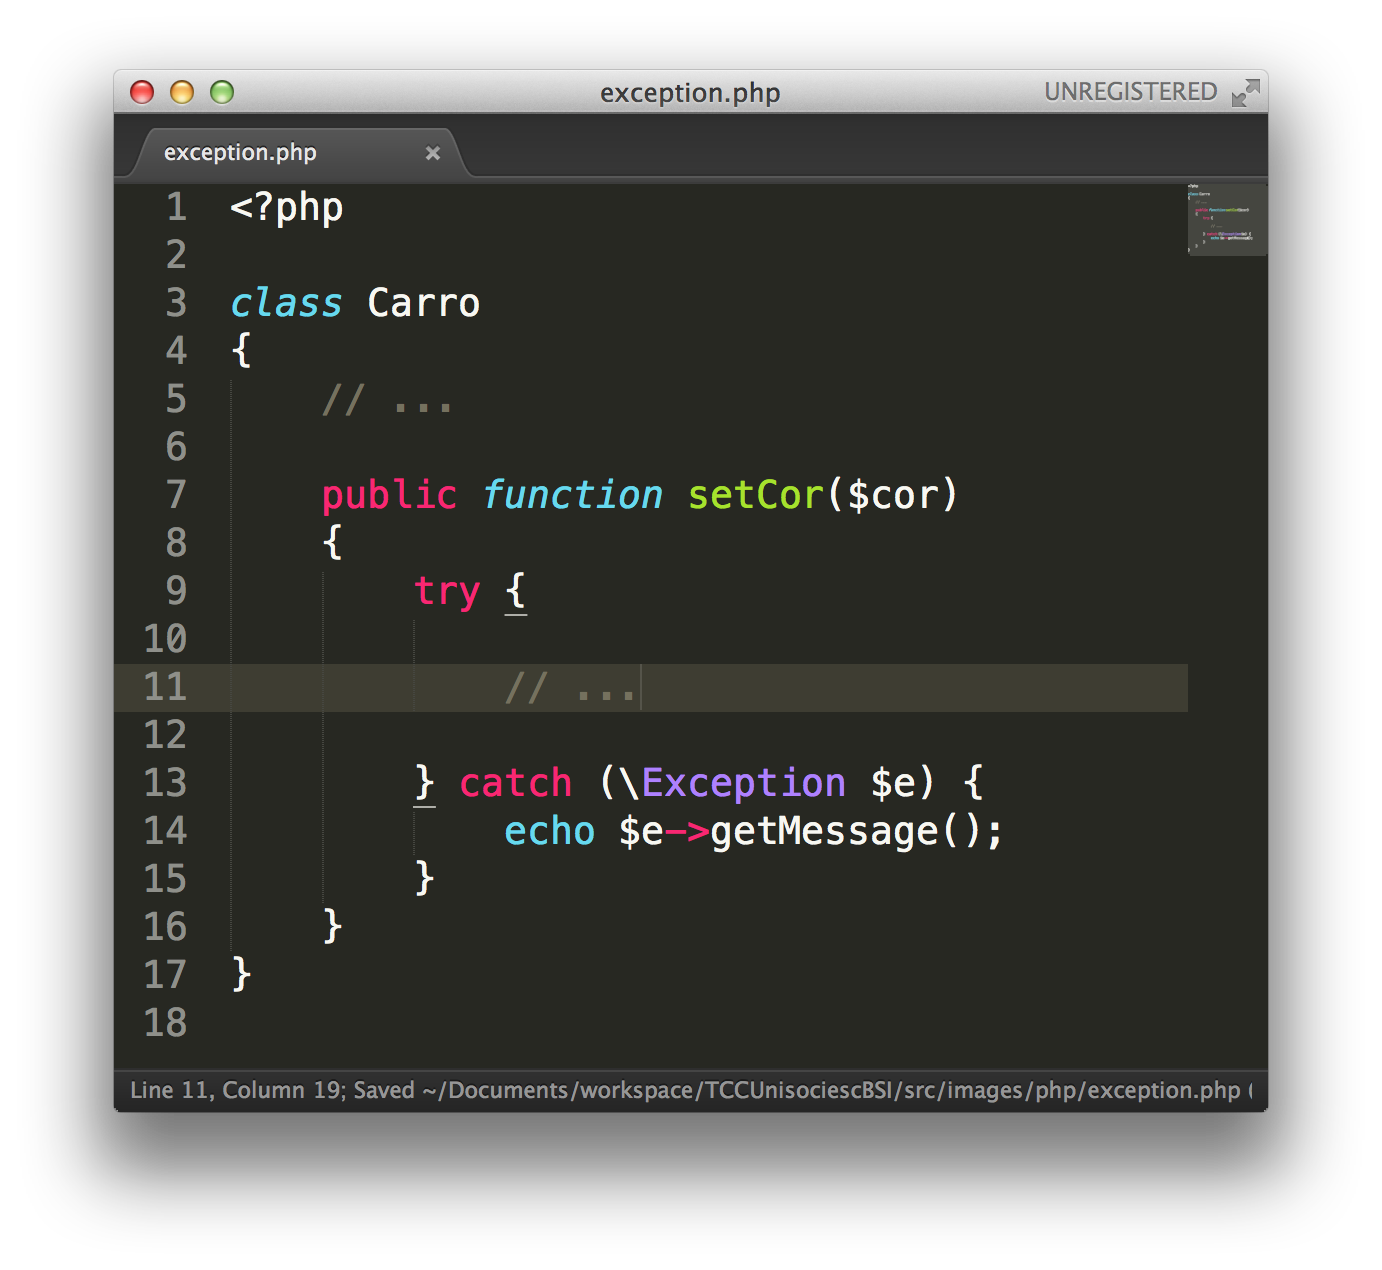
\includegraphics[width=0.75\textwidth]{images/exception.png}

	\centering
	\footnotesize Fonte: \fonteOAutor
\end{figure}

\FloatBarrier 	% Este comando impede que as imagens
				% flutuem a partir deste ponto no seu documento

A seguir, é apresentado em detalhes as linhas de código exibidas na Figura
\ref{fig:excecao}:

\begin{alineas}
    \item linha 7: define-se um método chamado \textit{setCor};
    \item linha 9: utiliza-se a palavra reservada \textbf{try} informando ao
    \acs{PHP} que o que estiver entre os delimitadores deste bloco pode não
    ocorrer de forma esperada, ou seja, tente realizar este procedimento;
    \item linha 13: caso ocorra algum problema na execução do \textit{script}
    definido na linha 11, o \acs{PHP} irá tratar o erro atribuindo-o a variável
    \textbf{\$e};
    \item linha 14: mostra uma mensagem descritiva com relação ao erro que acaba
    de ocorrer.
\end{alineas}

Em seguida, será apresentado o conceito de interfaces, que permitem definir
contratos de implementação entre as classes que o assinarem.
